\documentclass[border=2pt]{standalone}
\usepackage{tikz,amsmath}
\begin{document}
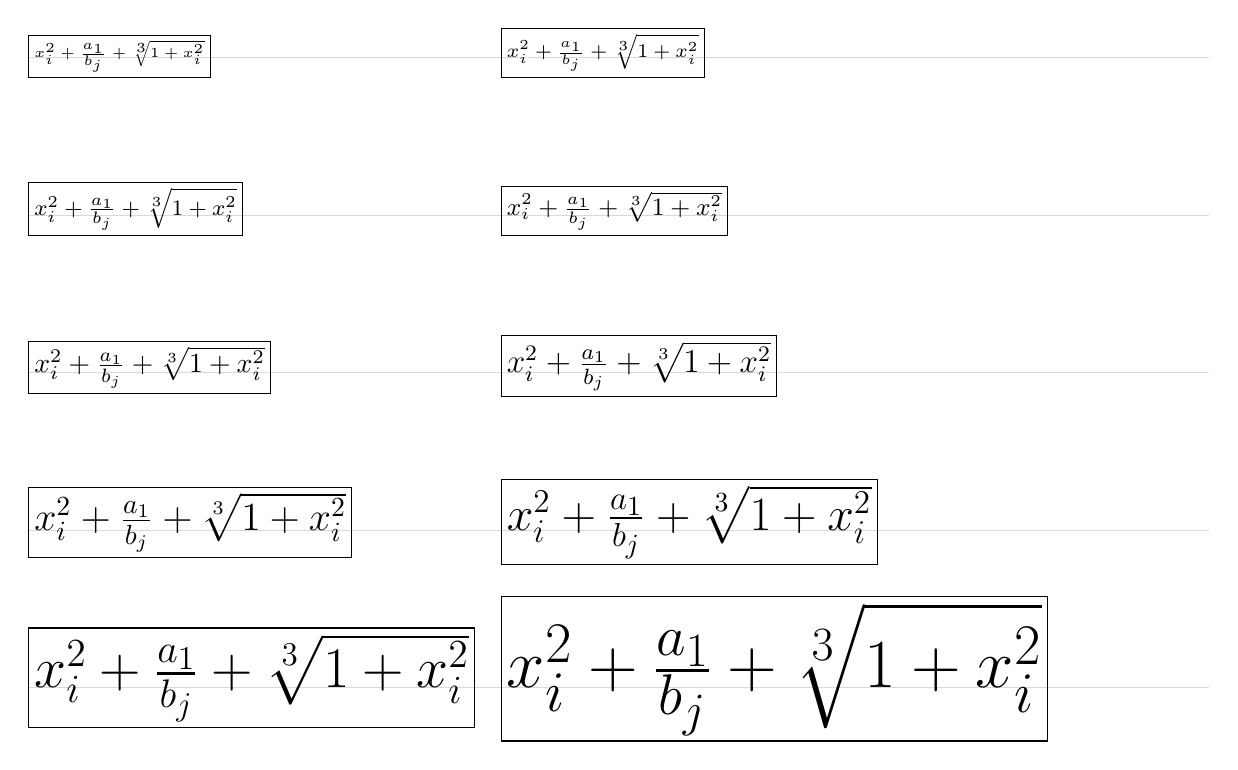
\begin{tikzpicture}
  \draw[gray!30] (0,0)--(15,0) (0,-2)--(15,-2) (0,-4)--(15,-4) (0,-6)--(15,-6) (0,-8)--(15,-8);
  \node[anchor=base west,draw,inner sep=2pt,font=\tiny] at (0,0) {$x_i^2+\frac{a_1}{b_j}+\sqrt[3]{1+x_i^2}$};
  \node[anchor=base west,draw,inner sep=2pt,font=\scriptsize] at (6,0) {$x_i^2+\frac{a_1}{b_j}+\sqrt[3]{1+x_i^2}$};
  \node[anchor=base west,draw,inner sep=2pt,font=\footnotesize] at (0,-2) {$x_i^2+\frac{a_1}{b_j}+\sqrt[3]{1+x_i^2}$};
  \node[anchor=base west,draw,inner sep=2pt,font=\small] at (6,-2) {$x_i^2+\frac{a_1}{b_j}+\sqrt[3]{1+x_i^2}$};
  \node[anchor=base west,draw,inner sep=2pt,font=\normalsize] at (0,-4) {$x_i^2+\frac{a_1}{b_j}+\sqrt[3]{1+x_i^2}$};
  \node[anchor=base west,draw,inner sep=2pt,font=\large] at (6,-4) {$x_i^2+\frac{a_1}{b_j}+\sqrt[3]{1+x_i^2}$};
  \node[anchor=base west,draw,inner sep=2pt,font=\Large] at (0,-6) {$x_i^2+\frac{a_1}{b_j}+\sqrt[3]{1+x_i^2}$};
  \node[anchor=base west,draw,inner sep=2pt,font=\LARGE] at (6,-6) {$x_i^2+\frac{a_1}{b_j}+\sqrt[3]{1+x_i^2}$};
  \node[anchor=base west,draw,inner sep=2pt,font=\huge] at (0,-8) {$x_i^2+\frac{a_1}{b_j}+\sqrt[3]{1+x_i^2}$};
  \node[anchor=base west,draw,inner sep=2pt,font=\Huge] at (6,-8) {$x_i^2+\frac{a_1}{b_j}+\sqrt[3]{1+x_i^2}$};
\end{tikzpicture}
\end{document}
